\section{Introduction}

When the data you want to model is high-dimensional, that is, the number of features \(p\)
exceed the number of observations \(n\), it is impossible to apply classical statistical
models such as standard linear regression since the design matrix \(\mat X\) is no longer
of full rank. A common remedy to this problem is to \emph{regularize} the model by adding a
term to the objective function that punishes models with large coefficients
(\(\vec\beta\)). If we let \(g(\vec\beta; \mat X, \vec y)\) be the original objective
function---which when minimized improves the model's fit to the data (\(\mat X, \vec
y\))---then
\begin{equation}
  \label{eq:general-objective}
  f(\beta_0, \vec\beta; \mat X, \vec y) = g(\beta_0, \vec\beta; \mat X, \vec y) + h(\vec\beta)
\end{equation}
is a composite function within which we have added a penalty term \(h(\vec\beta)\). In
contrast to \(g\), this penalty depends only on \(\vec{\beta}\). The intercept,
\(\beta_0\), is not typically penalized.

Some of the most common penalties are the \(\ell_1\) norm and squared \(\ell_2\) norm
penalties, that is \(h(\vec\beta) = \lVert \vec\beta \rVert_1\) or \(h(\vec\beta) = \lVert
\vec\beta \rVert_2^2/2\)\footnote{Division by two in this case is used only for
  convenience.}, which, if \(g\) is the standard ordinary least-squares objective, represent
lasso~\citep{tibshirani1996,santosa1986,donoho1994} and ridge (Tikhonov) regression
respectively. Other common penalities include SLOPE~\citep{bogdan2013,bogdan2015}, the
minimax-concave penalty (MCP)~\citep{zhang2010}, hinge loss (used in support vector
machines~\citep{cortes1995}) and smoothly-clipped absolute
deviation~(SCAD)~\citep{fan2001}. Many of these penalities---indeed all of the previously
mentioned ones---shrink coefficients in proportion to their sizes.

The issue with this type of shrinkage is that it is typically sensitive to the scales of
the features in \(\mat X\). A common remedy is to \emph{normalize} the features before
fitting the model by shifting and dividing each column by respective centering and scaling
factors. For some problems such factors arise naturally from knowledge of the problem at
hand. In most cases, however, they must be estimated from data. A common stategy, for
instance, is to translate by the mean of each feature and scale by the standard deviation,
which is called \emph{standardization}. Standardization along with most other popular
choices for of normalization are based only on the marginal distributions of the features.
Some types, such as the normalization applied in the adaptive lasso~\citep{zou2006},
however, are based on the conditional distributions of the features and the response.
Another reason for normalizing the features is to improve the performance and stability of
optimization algorithms used to fit the model. We will not cover this aspect in this paper,
but note that it is an important one.

In most sources and discussions on regularized methods, normalization is typically treated
as a preprocessing step---separate from modeling. As we will show in this paper, however,
the type of normalization used can have a critical effect on the estimated model, sometimes
leading to entirely different conclusions with regard to feature importance as well as
predictive performance. As a first example of this, consider \Cref{fig:realdata-paths},
which displays the lasso paths for four real data sets and two different types of
normalization. Each panel shows the union of the first five predictors picked under either
normalization scheme. The choice of normalization evidently has a significant impact on the
estimated models in most of these cases. For the \texttt{leukemia} data set, for instance,
the models are starkly different with respect to both the identities of the features
selected as well as their signs and magnitudes.

\begin{figure}[bpt]
  \centering
  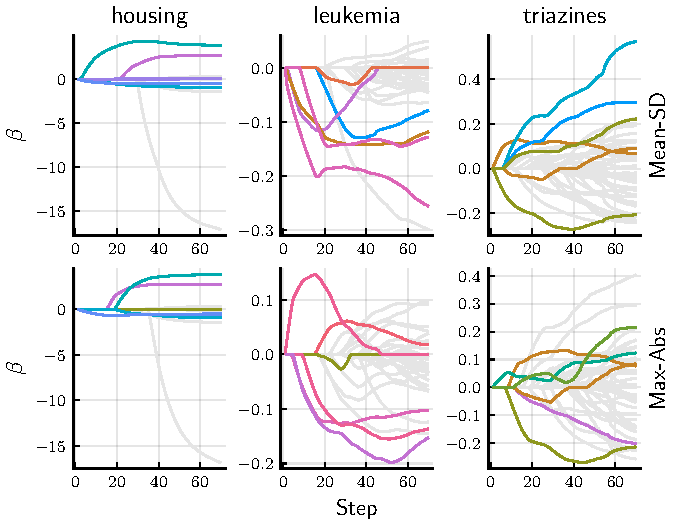
\includegraphics[]{plots/realdata_paths.pdf}
  \caption{%
    Lasso paths for real datasets using two types of normalization: standardization and maximum absolute value scaling (max--abs). We have fit the lasso path to four different datasets: \data{housing}~\citep{harrison1978}, \data{leukemia}~\citep{golub1999}, \data{triazines}~\citep{king}, and \data{w1a}~\citep{platt1998}. For each dataset, we have colored the coefficients if they were among the first five features to become active in under either of the two types of normalization schemes. We see that the paths differ with regards to the size as well as the signs of the coefficients, and that, in addition, the coefficients to become active first differ between the normalization types.
  }
  \label{fig:realdata-paths}
\end{figure}

% TODO: maybe put this paragraph the discussion instead
Recommendations for the choice of normalization are often based on computational aspects
and data storage requirements, rather than on the statistical properties of the choice of
normalization. At the time of writing, for instance, the popular machine learning library
\texttt{scikit-learn}~\citep{scikit-learndevelopers2024} recommends max--abs scaling in the
particular case of sparse data. We argue that this is misguided since basing the choice of
normalization on the type of data storage encodes a belief that the information in a data
set is somehow different if it is stored in a sparse viz-a-viz dense format. In constrast,
we believe that normalization should rather be considered an integral part of the model.

There are moreover many unexplored questions regarding what effect the choice of
normalization has for features of different types. In particular, there is no consensus on
how to normalize binary features---where observations take values 0 and 1. Nor is there, as
far as we have been able to ascertain, research that attempts to bridge this knowledge gap.
Anecdotal suggestions include not normalizing binary features at all, or to normalize them
as you would if it were continuous data.

In this paper, we will focus on three models that each correspond to a particular case of
\Cref{eq:general-objective}: the lasso, ridge, and elastic net~\citep{zou2005}. The latter
of these, the elastic net, is in fact a generalization of the previous two, and is the
optimization problem of minimizing the following objective function,
%
\begin{equation*}
  \underbrace{\frac{1}{2} \lVert \vec y - \beta_0 - \tilde{\mat{X}}\vec{\beta} \rVert^2_2}_{g(\beta_0, \vec{\beta}; \mat{X}, \vec{y})}  + \underbrace{\lambda_1 \lVert \vec\beta \rVert_1 + \frac{\lambda_2}{2}\lVert \vec \beta \rVert_2^2}_{h(\vec{\beta})}.
\end{equation*}
%
Setting \(\lambda_1 = 0\), we obtain the ridge regression objective, whilst setting
\(\lambda_2 = 0\), we get the lasso. All of these methods have become staples in the field
of statistics and machine learning and are accompanied by a large body of theoretical work
as well as numerous practical applications. In this paper, we will focus on how these
models are affected by the use of normalization when they are fit to binary features. We
pay particular attention to the case when these binary features are imbalanced, that is,
have relatively many ones or zeroes. In this case, we demonstrate that the choice of
normalization directly influences the size of the regression coefficients and that this
effect is different for the lasso and ridge regression. We also show how to mitigate this
effect to remove this class imbalance bias. In the case of the elastic net, however, we
show that there is no simple normalization method that can mitigate this bias and that we
instead need to consider weighting the penalty term in the elastic net.
